%% ----------------------------------------------------------------------------
%%  §11.7  Serie alternate
%% ----------------------------------------------------------------------------
\section{Serie alternate}
\label{sec:serie-alternate}

Finora abbiamo studiato quasi esclusivamente serie a termini non negativi. Eliminiamo
questa restrizione, cominciando dalle \emph{serie alternate}\index{serie!alternata},
cioè le serie del tipo
\begin{equation}\label{eq:serie-alternata}
  \sum_{k=1}^{\infty}(-1)^{k-1}a_{k}=a_{1}-a_{2}+a_{3}-a_{4}+\dots+(-1)^{n-1}a_{n}+\cdots, \qquad a_{n}\ge0 ,
\end{equation}
in cui i termini cambiano segno a ogni passo. L'esempio tipico è la \emph{serie armonica
alternata}
\begin{equation}\label{eq:armonica-alternata}
  \sum_{k=1}^{\infty}\frac{(-1)^{k-1}}k=1-\frac12+\frac13-\frac14+\cdots ,
\end{equation}
che, a differenza della serie armonica, converge. Il meccanismo è visibile nella
\cref{fig:alternata}: ogni termine «corregge» il precedente con una correzione più
piccola, e le somme parziali oscillano attorno alla somma con oscillazioni sempre più
strette. Ci servirà un semplice lemma sulle successioni.

\begin{lemma}\label{lem:pari-dispari}
Se le estratte di indici pari $s_{2k}$ e di indici dispari $s_{2k+1}$ di una successione
$s_{n}$ convergono allo stesso limite $s$, allora $s_{n}\to s$.
\end{lemma}

\begin{schema}
\Ipotesi{$s_{2k}\to s$ \ e \ $s_{2k+1}\to s$ per $k\to+\infty$, con $s\in\R$.}
\Tesi{$s_{n}\to s$.}
\end{schema}

\begin{strategia}
Ogni indice $n$ è pari o dispari. Fissato $\epsilon>0$, le due estratte entrano
definitivamente nell'intorno $(s-\epsilon,s+\epsilon)$, ciascuna da un proprio indice in poi: basta
prendere il più grande dei due indici, tradotto in termini di $n$.
\end{strategia}

\begin{dimostrazione}
Sia $\epsilon>0$. Esistono $k_{1}$ e $k_{2}$ tali che $\abs{s_{2k}-s}<\epsilon$ per $k>k_{1}$ e
$\abs{s_{2k+1}-s}<\epsilon$ per $k>k_{2}$. Posto $\nu=2\max\{k_{1},k_{2}\}+1$, ogni $n>\nu$ è della forma
$2k$ con $k>k_{1}$ oppure $2k+1$ con $k>k_{2}$, e in entrambi i casi $\abs{s_{n}-s}<\epsilon$.
\end{dimostrazione}

\begin{teorema}[Criterio di Leibniz]\label{teo:leibniz}\index{criterio di Leibniz}
Sia $a_{n}\ge0$ una successione decrescente e infinitesima. Allora la serie alternata
\eqref{eq:serie-alternata} è convergente. Inoltre, detta $s$ la sua somma e $s_{n}$ la
somma parziale $n$-esima, si ha
\begin{equation}\label{eq:stima-leibniz}
  \abs{s_{n}-s}\le a_{n+1} \qquad\perogni n\in\N ,
\end{equation}
e la somma $s$ è compresa tra due somme parziali consecutive qualsiasi.
\end{teorema}

\begin{schema}
\Ipotesi{$a_{n}\ge0$; \ $a_{n+1}\le a_{n}$ per ogni $n$; \ $a_{n}\to0$.}
\Tesi{$\sum(-1)^{k-1}a_{k}$ converge; \ $\abs{s_{n}-s}\le a_{n+1}$.}
\end{schema}

\begin{strategia}
Separiamo le somme parziali di indice pari da quelle di indice dispari. Passando da
$s_{2k}$ a $s_{2k+2}$ si aggiunge $a_{2k+1}-a_{2k+2}\ge0$: le somme pari crescono. Passando da
$s_{2k-1}$ a $s_{2k+1}$ si aggiunge $-a_{2k}+a_{2k+1}\le0$: le somme dispari decrescono. Inoltre
ogni somma dispari supera ogni somma pari. Abbiamo due successioni monotòne e
limitate, una che sale e una che scende, la cui distanza $a_{2k+1}$ tende a zero: come in una
successione di intervalli incapsulati, convergono allo stesso limite, che è compreso tra
loro. La stima dell'errore segue proprio da questo «incapsulamento».
\end{strategia}

\begin{dimostrazione}
Per ogni $k\in\N$, poiché $a_{n}$ è decrescente,
\begin{align}
  s_{2k+2}&=s_{2k}+(a_{2k+1}-a_{2k+2})\ge s_{2k} , \label{eq:leibniz-pari}\\
  s_{2k+1}&=s_{2k-1}-(a_{2k}-a_{2k+1})\le s_{2k-1} . \label{eq:leibniz-dispari}
\end{align}
Dunque $s_{2}\le s_{4}\le s_{6}\le\cdots$ e $s_{1}\ge s_{3}\ge s_{5}\ge\cdots$. Inoltre
$s_{2k+1}-s_{2k}=a_{2k+1}\ge0$, e quindi
\begin{equation}\label{eq:leibniz-incapsulati}
  s_{2}\le s_{2k}\le s_{2k+1}\le s_{1} \qquad\perogni k\in\N .
\end{equation}
La successione $s_{2k}$ è crescente e limitata superiormente da $s_{1}$, la successione
$s_{2k+1}$ è decrescente e limitata inferiormente da $s_{2}$; per il teorema sulle successioni
monotòne (\cref{teo:monotone}) esse convergono, a limiti $s'$ e $s''$. Passando al limite
in $s_{2k+1}-s_{2k}=a_{2k+1}$ si ottiene $s''-s'=0$, perché $a_{n}\to0$. Per il
\cref{lem:pari-dispari} la serie converge, e la sua somma è $s=s'=s''$.

Per il teorema sulle successioni monotòne, inoltre, $s=\sup_{k}s_{2k}=\inf_{k}s_{2k+1}$, e quindi
$s_{2k}\le s\le s_{2k+1}$ e $s\le s_{2k-1}$ per ogni $k$. Ne segue
\begin{align*}
  0&\le s-s_{2k}\le s_{2k+1}-s_{2k}=a_{2k+1} ,\\
  0&\le s_{2k+1}-s\le s_{2k+1}-s_{2k+2}=a_{2k+2} ,
\end{align*}
cioè $\abs{s_{n}-s}\le a_{n+1}$ sia per $n=2k$ sia per $n=2k+1$; per $n=1$ la stessa disuguaglianza
segue da $s_{2}\le s\le s_{1}$. Le disuguaglianze $s_{2k}\le s\le s_{2k\pm1}$ dicono anche che $s$ è
compresa tra due somme parziali consecutive.
\end{dimostrazione}

La \eqref{eq:stima-leibniz} si enuncia spesso così: \emph{per una serie alternata che
verifica le ipotesi del criterio di Leibniz, l'errore che si commette sostituendo alla
somma la somma dei primi $n$ termini è maggiorato, in valore assoluto, dal primo termine
trascurato}. Si sa anche il segno dell'errore: è quello del primo termine trascurato.

\begin{esempio}[La serie armonica alternata]\label{es:armonica-alternata}
La successione $a_{n}=\frac1n$ è positiva, decrescente e infinitesima: la serie
\eqref{eq:armonica-alternata} converge. Quanti termini occorre sommare per avere
$\abs{s-s_{n}}\le\frac1{100}$? Per la \eqref{eq:stima-leibniz} basta che $a_{n+1}=\frac1{n+1}\le\frac1{100}$,
cioè $n\ge99$. Il valore della somma si ottiene dallo sviluppo del logaritmo: nel
\S\ref{sec:taylor-peano} abbiamo visto che
$\log(1+x)=\sum_{k=1}^{n}\frac{(-1)^{k-1}}kx^{k}+R(x)$ con $\abs{R(x)}\le\frac{x^{n+1}}{n+1}$ per $x\ge0$. Con
$x=1$, $\abs{\log2-s_{n}}\le\frac1{n+1}\to0$, e dunque
\begin{equation}\label{eq:somma-log2}
  1-\frac12+\frac13-\frac14+\dots=\log2=0{,}693147\ldots
\end{equation}
Allo stesso modo la serie di Leibniz \eqref{eq:serie-leibniz},
$1-\frac13+\frac15-\cdots=\frac\pi4$, verifica le ipotesi del criterio, e la stima
$\abs{s_{n}-\frac\pi4}\le\frac1{2n+1}$ ritrova quella del \cref{cap:taylor}.
\end{esempio}

\begin{attenzione}
L'ipotesi che $a_{n}$ sia \emph{decrescente} non si può omettere. Si consideri la serie
alternata con $a_{2j-1}=\frac1j$ e $a_{2j}=\frac1{4j^{2}}$:
\[
  1-\frac14+\frac12-\frac1{16}+\frac13-\frac1{36}+\cdots .
\]
I termini tendono a zero, ma non in modo monotòno. Le somme parziali di indice pari sono
$s_{2m}=\sum_{j=1}^{m}\bigl(\frac1j-\frac1{4j^{2}}\bigr)=H_{m}-\frac14\sum_{j=1}^{m}\frac1{j^{2}}$, che tende a $+\infty$
perché $H_{m}\to+\infty$ mentre $\sum\frac1{j^{2}}$ converge. Anche $s_{2m+1}=s_{2m}+\frac1{m+1}>s_{2m}$ tende a
$+\infty$, e per il \cref{lem:pari-dispari} (che vale, con la stessa dimostrazione e con gli
intorni di $+\infty$ al posto di quelli di $s$, anche per limiti infiniti) la serie diverge.
\end{attenzione}

\begin{figure}[htb]
\centering
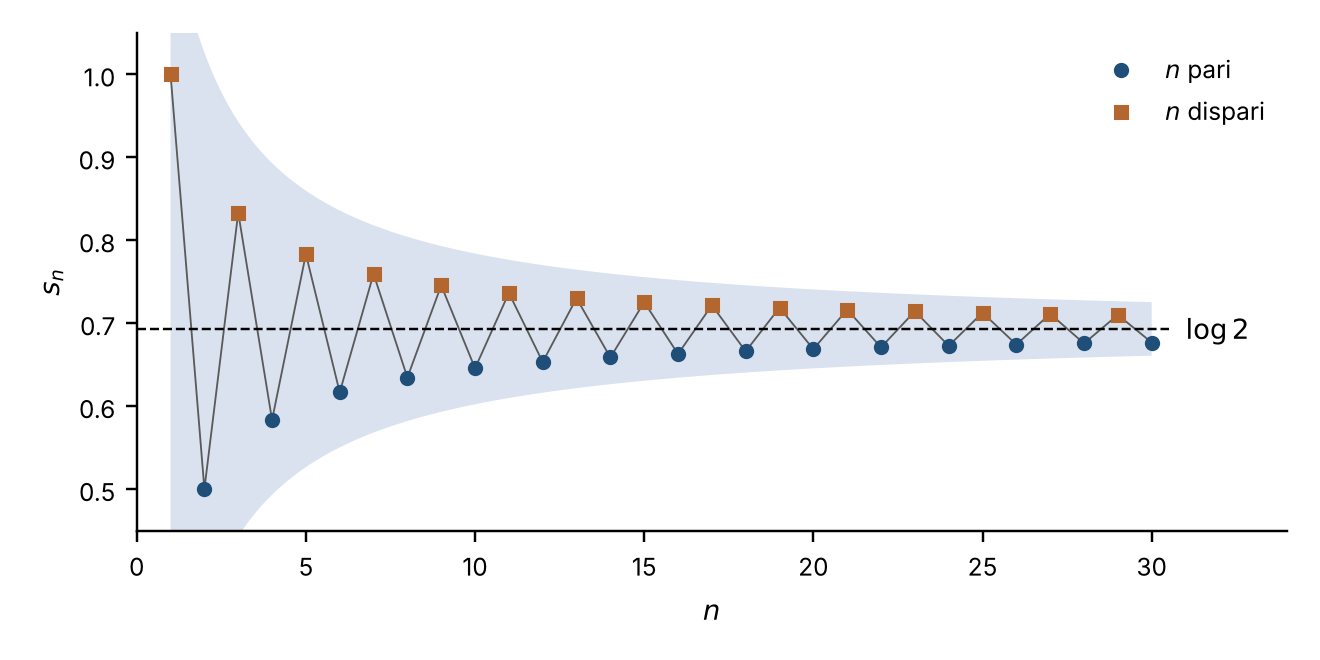
\includegraphics[width=\textwidth]{figure/alternata.png}
\caption{Le somme parziali della serie armonica alternata (punti) oscillano attorno alla
somma $\log2$: quelle di indice pari crescono, quelle di indice dispari decrescono, e la
somma è sempre compresa tra due somme consecutive. La fascia grigia ha semiampiezza
$a_{n+1}=\frac1{n+1}$, la stima dell'errore del criterio di Leibniz
(\texttt{python/fig\_alternata.py}).}
\label{fig:alternata}
\end{figure}

\needspace{10\baselineskip}
\begin{python}[La serie armonica alternata]
import math

s, err_max = 0.0, 0.0
for n in range(1, 10001):
    s += (-1)**(n - 1) / n
    errore = abs(s - math.log(2))
    err_max = max(err_max, errore * (n + 1))   # errore / a_(n+1)
    if n in (10, 99, 100, 1000, 10000):
        print(f"n = {n:5d}: s_n = {s:.8f}  errore = {errore:.2e}"
              f"  a_(n+1) = {1/(n+1):.2e}")
print(f"max di |s_n - log 2| / a_(n+1) = {err_max:.4f}  (<= 1)")
\end{python}
\begin{risultato}
n =    10: s_n = 0.64563492  errore = 4.75e-02  a_(n+1) = 9.09e-02
n =    99: s_n = 0.69817218  errore = 5.02e-03  a_(n+1) = 1.00e-02
n =   100: s_n = 0.68817218  errore = 4.98e-03  a_(n+1) = 9.90e-03
n =  1000: s_n = 0.69264743  errore = 5.00e-04  a_(n+1) = 9.99e-04
n = 10000: s_n = 0.69309718  errore = 5.00e-05  a_(n+1) = 1.00e-04
max di |s_n - log 2| / a_(n+1) = 0.6137  (<= 1)
\end{risultato}
